\documentclass{classes/sice-si}


% \title{
% 	カーリングスキップロボットに関する研究 ~第一報:LRFとカメラを用いたストーン検出とシステムのROS化~
% }

% \author{
% 	〇熊本涼介,Trinh Quang Phi,曽根忠瑛,河村隆
% }

% タイトルと著者名
\title{カーリングストーンデリバリロボットにおける回転付加機構に関する検討と実装} % 和文タイトル
\name{○伊與田一,曽根忠瑛,河村隆(信州大学)} % 著者名
\etitle{Study and Implementation of Rotational Addition Mechanism in Curling Stone Delivery Robot} % 英文タイトル
\ename{○Hajime IYODA,Tadaaki SONE and Takashi KAWAMURA \\Shinshu University}	%著者名(英)


\setlength\textfloatsep{0pt} % 図と本文の間のスペース
\setlength\floatsep{0pt} % 図同士の間のスペース
\setlength\intextsep{0pt} % 図と本文の間のスペース(本文中の図の場合)

\begin{document}

% アブストラクト
\abst{人間にはできない再現性のある投球を行うカーリングストーンデリバリロボットの
開発を行っている。
デリバリロボットの重要な機構の一つである回転付加機構の検討と実装について述べる。
    % In order to estimate the position of stones around a curling House with high accuracy, LRF and
    % camera-equipped skip robot system is being developed.
    % The LRF gets relatively accurate data of stone positions, and the camera obtains overview data.
    % Build a ROS 2 system to measure the stone's position from LRF and camera sensor data.
    % The curling tactical AI recieve the position data to use for tactical planning.
}



\maketitle

\section{緒言}
本研究は,カーリング競技を対象とする.カーリング競技は,1998 年の長野大会からオリ
ンピックの正式競技に採用され,2022 年の北京オリンピックにて,日本史上初となる銀メダ
ルを獲得し ,日本国内でも広く認知される有名競技となった.
しかし,ウィンタースポーツ全体で見ると,日本における競技人口は2020 年の調査では,
登録競技者が全体で2306 人と少なく,また施設の普及の点においても他の競技には及ば
ない,その理由として競技の理解が進んでいないことが原因の一つとして挙げられる.カー
リングは「氷上のチェス」と呼ばれ,細かい戦略,高度な技術を要するスポーツである.
氷の状態を読みストーンの投球を行うことは人の経験や感覚に頼る
ことが多く,戦略も大まかな定石しか存在しない.また,カーリングが行える環境が少ない
ことも普及の妨げになっていると考える.日本カーリング協会によると,カーリング専用施
設は2024 年現在で日本に13 箇所しかなく,通年で使用可能な施設は8 箇所に限られる.
試合が行われるフィールド(カーリングシート)にも,製作や整備(アイスメイク)にも専
門的な技術を要する.

本研究の目的は,人間と対戦可能なカーリングロボットシステムを開発することで,ストーンの挙動に関する物理現象を解明し,カーリング競技の普及・発展に寄与することである.
本報では,カーリングストーンデリバリロボットにおける回転付加機構に関する検討と実装について述べる.
\section{回転付加機構について}
回転付加機構は,ストーンに角速度を与える機構であり,目標角速度は約12 rpmである.ストーンに回転を与えることにより,ストーンはカール(曲がる)する.


\subsection{先行研究について}
これまでに開発された回転付加機構について述べる.
先行研究では3つの回転付加機構が考案され、開発された
\begin{itemize}
    \item 平ベルト方式 \mbox{}\\
    モータに取り付けられたプーリで平ベルトを駆動させ,ストーンを押し出した際にベルトとストーンが接触し,摩擦によってストーンを回転させる
    \item ウレタンローラ方式\mbox{}\\
    モータに取り付けられたウレタンローラでストーンを回転させ,ストーンを回転させる。
    \item タイミングベルト方式\mbox{}\\
    平ベルト式を参考にし開発され、問題を解決するために開発された。
    モータに取り付けられたプーリでタイミングベルトを駆動させ,ストーンを押し出した際にベルトとストーンが接触し,摩擦によってストーンを回転させる
\end{itemize}
しかし、先行研究の回転付加機構には問題が残されている
\begin{description}
    \item 確実な回転ができていない問題
    \item 部品の剛性が低い問題
\end{description}
これらの問題が残されているため、新たな回転付加機構の開発が必要である。

\begin{figure}[H]
    \centering
    \vspace{4pt} % 上部の余白を0に設定
    \begin{minipage}{0.45\linewidth}
        \centering
        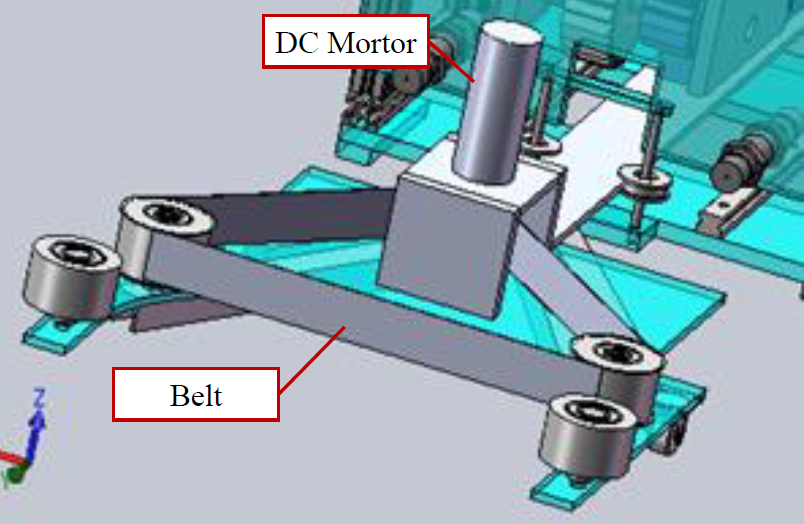
\includegraphics[width=\linewidth]{figures/1.png}
        \caption{Clustering by LRF}
        \label{fig:1}
    \end{minipage}
    \hfill
    \begin{minipage}{0.45\linewidth}
        \centering
        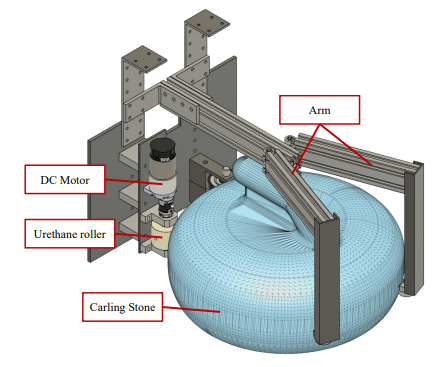
\includegraphics[width=\linewidth]{figures/2.png}
        \caption{Matching by LRF}
        \label{fig:2}
    \end{minipage}
    \hfill
    \begin{minipage}{0.45\linewidth}
        \centering
        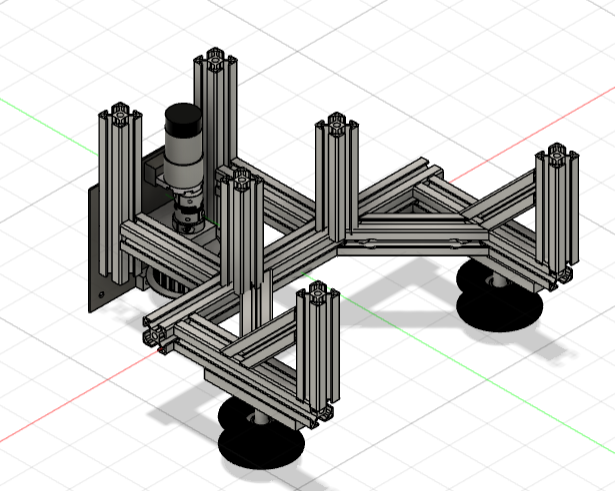
\includegraphics[width=\linewidth]{figures/3.png}
        \caption{Matching by LRF}
        \label{fig:3}
    \end{minipage}
    \vspace{0pt} % 上部の余白を0に設定
\end{figure}
\subsection{新型回転付加機構の開発}
開発された,回転付加機構について述べる.先行研究で開発された回転付加機構の改善を行い,問題点の解決を図った.
現在設計を行っている回転付加機構のCAD図を図\ref{fig:new}に示す.
問題解決のために,カーリングストーンのハンドルを保持し,ストーンを回転させる機構を設計を行っている.

\begin{figure}[H]
    \centering
    \begin{minipage}{0.7\linewidth}
        \centering
        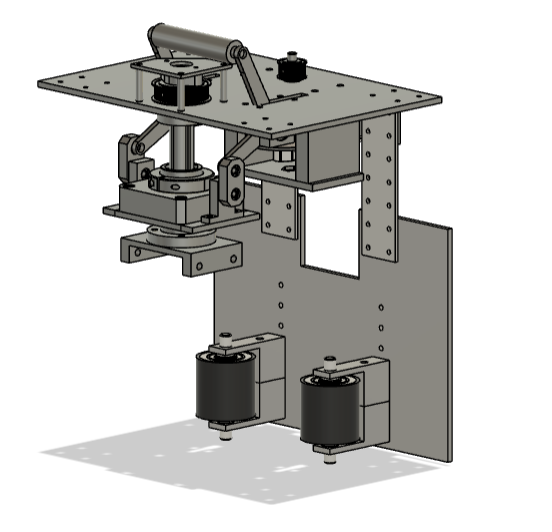
\includegraphics[width=\linewidth]{figures/4.png}
        \caption{Clustering by LRF}
        \label{fig:new}
    \end{minipage}
    \hfill
    \vspace{0pt} % 上部の余白を0に設定
\end{figure}



\section{結言}



% %参考文献
% % \begin{thebibliography}{99}
    % % \bibitem{SI}
    % % 計測太郎,制御花子:
    % % ``SICE SI予稿原稿の書き方(サンプル)'',
    % % {\it 計測自動制御学会SI部門講演会SICE-SI予稿集},
    % % pp.0000--0000 (20??)
    % % \end{thebibliography}

\printbibliography[title=参考文献]





\end{document}